\documentclass[xcolor = {dvipsnames, table}, aspectratio=169]{beamer}

\definecolor{dotlightblue} {HTML}{ADD8E6}
\definecolor{dotlightcoral}{HTML}{F08080}

\RequirePackage[english]{babel}
\RequirePackage[utf8]{inputenc}

\RequirePackage{fancyvrb}
\RequirePackage{tabularx}

\RequirePackage{listings}
\lstset{
    language = C,
    basicstyle = \ttfamily,
}

% \set{}
\RequirePackage{braket}

\RequirePackage{amsmath}

\RequirePackage{tikz}
% for arrows inside listings
\usetikzlibrary{decorations.text, calc}
\usetikzlibrary{positioning, matrix, arrows.meta}
\newcommand{\tikzmark}[2]{%
     \tikz[overlay,remember picture]%
        \node[text=black, inner sep=2pt] (#1) {#2};%
}

\RequirePackage{pgfplots}
\pgfplotsset{compat = newest}

\RequirePackage{algorithm}
\RequirePackage[noend]{algpseudocode}

\algnewcommand \algorithmicin{\textbf{in}}
\algnewcommand \In {\algorithmicin\ }
\algnewcommand \algorithmiccontinue{\textbf{continue}}
\algnewcommand \Continue {\State \algorithmiccontinue\ }
\algnewcommand \algorithmicskip{\textbf{skip}}
\algnewcommand \Skip {\State \algorithmicskip\ }
\algrenewtext{ForAll}[2]%
    {\algorithmicfor\ #1 \algorithmicin\ #2 \algorithmicdo}
\algnewcommand \SkipIf[1] {\State \algorithmicskip\ \algorithmicif\ #1}

% reduce the size of the font in algorithms slightly
\makeatletter
\renewcommand{\ALG@beginalgorithmic}{\footnotesize}
\makeatother

\AtBeginSection[]{
    \begin{frame}
        \vfill
        \centering
        \begin{beamercolorbox}[sep=8pt,center,shadow=true,rounded=true]{title}
            \usebeamerfont{title}\insertsectionhead\par%
        \end{beamercolorbox}
        \vfill
    \end{frame}
}

% https://tex.stackexchange.com/questions/142672/uncovering-lines-in-an-equation-in-split-environment
\newcommand{\disponslide}[2]{%
    \alt<#1>{#2}{\phantom{#2}}
}

%Information to be included in the title page:
\title{MC/DC in gcc}
\author{Jørgen Kvalsvik j@lambda.is}
\date{20/04/2023}

\begin{document}
{
\usebackgroundtemplate{\includegraphics[height=\paperheight]{accu-cover.png}}
    \begin{frame}[plain] \end{frame}
}

\begin{frame}
    \begin{block}{Topics}
        \begin{itemize}
            \item Code coverage - overview and taxonomy
            \item Introduction to modified condition/decision coverage (MC/DC)
            \item Some example programs
            \item A (thorough) description of the algorithm in gcc (notation warning)
        \end{itemize}
    \end{block}
\end{frame}

\begin{frame}
    \begin{block}{By the end you will ...}
        \begin{itemize}
            \item Be familiar with \{line, branch, condition\} coverage
            \item Know about different kinds of MC/DC
            \item Understand masked conditions
            \item Be able to measure MC/DC with gcc and gcov
            \item Have seen some cool maths
        \end{itemize}
    \end{block}

    There will also be some nuggets, words of wisdom, from smart people
    % TODO: disclaimer: using a lot of examples which could be caught in unit
    % tests, but would apply to more subtle interactions
\end{frame}

\section{Code coverage}
\begin{frame}
    Code coverage is a \textbf{collection of metrics} for different properties
    of your \textbf{test suite}. Programs are \textbf{instrumented} to record
    \textbf{run-time} information. This is sensitive to inputs and results are
    usually aggregated over \textbf{multiple runs}.
\end{frame}

\begin{frame}
    \begin{block}{Nugget}
        Any coverage metric should not be a \textbf{goal}, but a measurement of
        how well the \textbf{requirement tests} exercise the structure of
        the program.
    \end{block}

    \begin{block}{}
        \small{
            Hayhurst (2001): A Practical Tutorial on Modified Condition/
            Decision Coverage.
        }
    \end{block}
\end{frame}

\begin{frame}[fragile]
    Silly example:

    \begin{lstlisting}[language = C]
bool maybe_record(double a) {
    if (round(a) >= a) {
        update_counter();
        return true;
    } else {
        return false;
    }
}
maybe_record(0.6); // should round up
maybe_record(6.0); // should not round up
\end{lstlisting}
\end{frame}

\begin{frame}[fragile]
    \begin{lstlisting}
    2:    9:bool maybe_round(double x) {
    2:   10:    if (round(x) >= x) {
    2:   11:        update_counter();
    2:   12:        return true;
    -:   13:    } else {
#####:   14:        return false;
    -:   15:    }
    -:   16:}
    -:   17:
    1:   18:int main() {
    1:   19:    maybe_round(0.6);
    1:   20:    maybe_round(6.0);
    1:   21:}
    \end{lstlisting}
    Oops, else-block not exercised.
\end{frame}

\begin{frame}
    \begin{block}{A taxonomy of coverage metrics}
    \end{block}

    \begin{block}{}
        \begin{tabularx}{\textwidth}{l X}
            Line/Statement &
                Has every \textbf{line} of the source been executed? \\
            Branch/Decision &
                Has every \textbf{control flow} structure been evaluated to
                \emph{both} true and false? \\
            Condition &
                Has every \textbf{boolean sub-expression} been evaluated to
                \emph{both} true and false? \\
            %TODO: add later
            %Modified Condition/Decision coverage &
            %    Has every \textbf{control flow} structure been evaluated to
            %    \emph{both} true and false \textbf{and} every condition been shown
            %    to affect the decision outcome \textbf{independently}? \\
        \end{tabularx}
    \end{block}

    \pause
    Even line coverage can require a lot of effort
\end{frame}

\begin{frame}[fragile]
    \begin{block}{Line/Statement coverage}
        Has every \textbf{line} of the source been executed?
    \end{block}

    \begin{lstlisting}[language = C]
int badadder(int x, int y) {
    int tmp = x;
    tmp = tmp + (y - 5);
    return tmp;
    tmp += 5;  // dead as a do-do
}
    \end{lstlisting}

    Obviously cannot achieve 100\% line coverage.
\end{frame}

\begin{frame}[fragile]
    \begin{block}{Line/Statement coverage}
        Has every \textbf{line} of the source been executed?
    \end{block}

    \begin{lstlisting}[language = C]
int fn(T* x) {
    if (precondition1(x))
        return -1;
    if (precondition2(x))
        return -1;
    work(x);
    return 0;
}
    \end{lstlisting}
\end{frame}

\begin{frame}[fragile]
    \begin{block}{Branch/Decision coverage}
        Has every \textbf{control flow} structure been evaluated to \emph{both}
        true and false?
    \end{block}

    \begin{lstlisting}[language = C]
if (x) {
    // at least once
    first();
} else {
    // at least once
    second();
}
    \end{lstlisting}

    \pause
    \begin{block}{}
        How is this different from statement coverage?
    \end{block}
\end{frame}

\begin{frame}[fragile]
    \begin{onlyenv}<1>
        \begin{lstlisting}[language = C]
if (x) {
    first();
}
next();
        \end{lstlisting}
    \end{onlyenv}%
    \begin{onlyenv}<2>
        \begin{lstlisting}[language = C]
if (always_true()) {
    first();
}
next();
        \end{lstlisting}
    \end{onlyenv}%

    \visible<1>{When \lstinline{x} is \lstinline{true} this has 100\% statement
    coverage and 50\% decision coverage.}
\end{frame}

\begin{frame}[fragile]
    \begin{block}{every \textbf{control flow} [...]}
        \lstinline{for} and \lstinline{while} are \lstinline{if}s with fake
        beards
    \end{block}

    \begin{columns}
        \begin{column}{0.5\textwidth}
            \begin{lstlisting}[language = C, basicstyle = \scriptsize\ttfamily]
while (cond) {
    f(); g();
}
reset();
loop:
    if (!cond) goto endloop;
    f(); g();
    goto loop;
endloop: ;
            \end{lstlisting}
        \end{column}

        \begin{column}{0.5\textwidth}
            \begin{visibleenv}<2>
                \begin{lstlisting}[language = C, basicstyle = \tiny\ttfamily]
1:    6:int main() {
2:    7:    while (cond) {
branch  0 taken 50%
branch  1 taken 50% (fallthrough)
1:    8:        f(); g();
-:    9:    }
1:   10:    reset();
2:   11:loop:
2:   12:    if (!cond) goto endloop;
branch  0 taken 50% (fallthrough)
branch  1 taken 50%
1:   13:    f(); g();
1:   14:    goto loop;
1:   15:endloop: ;
-:   16:}
                \end{lstlisting}
            \end{visibleenv}
        \end{column}
    \end{columns}
\end{frame}

\begin{frame}[fragile]
    \begin{block}{Condition coverage}
        Has every \textbf{boolean sub-expression} been evaluated to
        \emph{both} true and false?
    \end{block}

    \begin{block}{}
        \begin{columns}
            \begin{column}{0.5\textwidth}
                \begin{lstlisting}[language = C]
    if (x && y) {
        both();
    }
                \end{lstlisting}
            \end{column}
            \begin{column}{0.5\textwidth}
                \begin{tabular}{c c c}
                    x & y & \%  \\
                    \hline
                    0 & 0 & 25  \\
                    1 & 0 & 75  \\
                    1 & 1 & 100 \\
                \end{tabular}
            \end{column}
        \end{columns}
    \end{block}
\end{frame}

\begin{frame}[fragile]
    \begin{block}{More statement vs decision coverage}
        \begin{lstlisting}[language = C]
while (accidently_always_true()) {
    f();
    if (g()) break;
    h();
}
        \end{lstlisting}
    \end{block}
\pause
The \textbf{loop} always terminates, but only because of the \textbf{break}.
Could have 100\% statement coverage, but not decision coverage.
\end{frame}

\begin{frame}[fragile]
    \begin{block}{More condition coverage}
        \begin{lstlisting}[language=C]
if (x && accidently_always_true(y)) {
    both();
} else {
    htob();
}

fn(0, 0); // 25%
fn(1, 0); // 75%
fn(1, 1); // 100%
        \end{lstlisting}
    \end{block}

    Condition coverage is clearly insufficient.
\end{frame}

\begin{frame}[fragile]
    \begin{lstlisting}[basicstyle=\scriptsize\ttfamily]
        $ gcov -b program
        3:    5:void fn(int x, int y) {
        3:    6:    if (x && accidently_always_true(y)) {
branch  0 taken 67% (fallthrough)
branch  1 taken 33%
branch  3 taken 100% (fallthrough)
branch  4 taken 0%
        2:    7:        both();
        -:    8:    } else {
        1:    9:        htob();
        -:   10:    }
        3:   11:}
        -:   12:
        1:   13:int main() {
        1:   14:    fn(0, 0);
        1:   15:    fn(1, 0);
        1:   16:    fn(1, 1);
        -:   17:}
    \end{lstlisting}
\end{frame}

\begin{frame}[fragile]
    \begin{block}{}
        \begin{lstlisting}[language = C++, basicstyle=\scriptsize\ttfamily]
struct C {
    C() { ... }
    C(const C&) { ... }
    C(C&&)      { ... }
    C& operator = (const C&) { ... }
    C& operator = (C&&)      { ... }
};
        \end{lstlisting}
    \end{block}

    \pause
    Does your test suite \emph{actually} call the move constructor?
\end{frame}

\begin{frame}
    \begin{block}{Nugget}
        \emph{C++ is the only language I know that lets you specify a custom
        copy function and then do its best to not call it.}
    \end{block}
    Tony van Eerd
\end{frame}

\section{gcc}

\begin{frame}
    gcc emits \textbf{.gcno} files (source annotation) and runs create or
    update \textbf{.gcda} files (counters)
\end{frame}

\begin{frame}
    \begin{block}{Quick start}
        \begin{itemize}
            \item Build with \lstinline{gcc --coverage}
            \item Run program, test suite
            \item Generate report with \lstinline{gcov <program>} or
                \lstinline{gcov <source>}
            \item Read the manual
        \end{itemize}
    \end{block}
\end{frame}

\begin{frame}
    \begin{block}{General advice}
        \begin{itemize}
            \item lcov is very useful
            \item Results (particularly source mapping) only reliable without
                optimizations
            \item Apply common sense and good engineering
        \end{itemize}
    \end{block}
\end{frame}

\section{Modified condition/decision coverage}

\begin{frame}
    \begin{itemize}
        \item How is it different from condition coverage?
        \item Why even care?
    \end{itemize}
\end{frame}

\begin{frame}
    Why even care?
    \begin{columns}
        \begin{column}{0.5\textwidth}
            \includegraphics[width = \textwidth]{img/bureaucrat.png}
        \end{column}

        \begin{column}{0.5\textwidth}
            \begin{itemize}
                \item DO-178B/C (Level A)
                \item ISO26262 (ASIL D)
            \end{itemize}
        \end{column}
    \end{columns}
\end{frame}

\begin{frame}
    Why even care?
    \begin{itemize}
        \item It is a good metric
        \item Can detect unintended data dependence
        \item Can detect classes of bad expressions
        \item Requires testing more interactions in your program
        \item Drives robustness
    \end{itemize}
\end{frame}

\newcommand \rowhl  {\rowcolor{Cyan!20}}
\newcommand \cellhl {\cellcolor{Cyan!20}}
\newcolumntype {C}{>{\columncolor{Cyan!20}}c}

\begin{frame}[fragile]
    The problem with decision coverage:
    \begin{columns}
        \begin{column}{0.5\textwidth}
            \begin{lstlisting}
if ((a && b) || c) {
    //
} else {
    //
}
            \end{lstlisting}
        \end{column}

        \begin{column}{0.5\textwidth}
            \begin{tabular}{c c c | c}
                        a & b & c \\
                        \hline
                \rowhl  F & F & F & F \\
                \rowhl  F & F & T & T \\
                        F & T & F & F \\
                        F & T & T & T \\
                        T & F & F & F \\
                        T & F & T & T \\
                        T & T & F & T \\
                        T & T & T & T \\
            \end{tabular}
        \end{column}
    \end{columns}

    \begin{block}{}
        Metric not very sensitive to the conditions and their interaction, only
        need two tests for three parameters.
    \end{block}
\end{frame}

\begin{frame}
    Modified condition/decision coverage satisfied if:
    \begin{itemize}
        \item every entry and exit point has been invoked
        \item every basic condition has taken on all possible outcomes
        \item each basic condition has been shown to independently affect the
              decision’s outcome
    \end{itemize}
\end{frame}

\begin{frame}[fragile]
    \begin{columns}
        \begin{column}{0.7\textwidth}
            \begin{lstlisting}[basicstyle = \footnotesize\ttfamily]
if ((a && b) || c) {
    //
} else {
    //
}
            \end{lstlisting}

            \begin{itemize}
                \item every entry and exit point has been invoked
            \end{itemize}

            Branch coverage
        \end{column}

        \begin{column}{0.3\textwidth}
            \begin{tabular}{c c c | c}
                        a & b & c \\
                        \hline
                \rowhl  F & F & F & F \\
                \rowhl  F & F & T & T \\
                        F & T & F & F \\
                        F & T & T & T \\
                        T & F & F & F \\
                        T & F & T & T \\
                        T & T & F & T \\
                        T & T & T & T \\
            \end{tabular}
        \end{column}
    \end{columns}
\end{frame}

\begin{frame}[fragile]
    \begin{columns}
        \begin{column}{0.7\textwidth}
            \begin{lstlisting}[basicstyle = \footnotesize\ttfamily]
if ((a && b) || c) {
    //
} else {
    //
}
            \end{lstlisting}
            \begin{itemize}
                \item every basic condition has taken on all possible outcomes
            \end{itemize}

            Condition coverage
        \end{column}

        \begin{column}{0.3\textwidth}
            \begin{tabular}{c c c | c}
                        a & b & c \\
                        \hline
                \rowhl  F & F & F & F \\
                        F & F & T & T \\
                        F & T & F & F \\
                        F & T & T & T \\
                        T & F & F & F \\
                \rowhl  T & F & T & T \\
                \rowhl  T & T & F & T \\
                        T & T & T & T \\
            \end{tabular}
        \end{column}
    \end{columns}
\end{frame}

\begin{frame}[fragile]
    \begin{columns}
        \begin{column}{0.7\textwidth}
            \begin{lstlisting}[basicstyle = \footnotesize\ttfamily]
if ((a && b) || c) {
    //
} else {
    //
}
            \end{lstlisting}
            \begin{itemize}
                \item each basic condition has been shown to
                      \emph{independently} affect the decision’s outcome
            \end{itemize}
            Modified condition/decision coverage
        \end{column}

        \begin{column}{0.3\textwidth}
            \begin{tabular}{c c c | c}
                        a & b & c \\
                        \hline
                \rowhl  F & F & F & F \\
                \rowhl  F & F & T & T \\
                        F & T & F & F \\
                        F & T & T & T \\
                \rowhl  T & F & F & F \\
                        T & F & T & T \\
                \rowhl  T & T & F & T \\
                        T & T & T & T \\
            \end{tabular}
        \end{column}
    \end{columns}
\end{frame}

\begin{frame}
    \begin{itemize}
        \item Testing all $2^N$ inputs would not reliably catch more defects
        \item $N+1$ test cases is sufficient (for coverage)
    \end{itemize}
\end{frame}

\begin{frame}
    The problem with MC/DC

    \begin{itemize}
        \item Only tests implementation, not the spec
        \item Possible to cheat
        \item Needs many test cases in maybe uninteresting places
        \item \emph{Awful} to determine without tooling
        \item Can be expensive and at odds with fuzzing
        \item Can lead to \emph{Metric Driven Development} (MDD)
    \end{itemize}
\end{frame}

\begin{frame}
    \begin{block}{Nugget}
        This is because MC/DC testing discourages defensive code with
        unreachable branches, but without defensive code, a fuzzer is more
        likely to find a path that causes problems.
    \end{block}

    \begin{block}{Nugget}
         MC/DC testing seems to work well for building code that is robust
         during normal use, whereas fuzz testing is good for building code that
         is robust against malicious attack.
    \end{block}

    \begin{block}{}
        https://www.sqlite.org/testing.html
    \end{block}
\end{frame}

\begin{frame}
    \begin{block}{A taxonomy of coverage metrics}
    \end{block}

    \begin{block}{}
        \begin{tabularx}{\textwidth}{l X}
            Line/Statement &
                Has every \textbf{line} of the source been executed? \\
            Branch/Decision &
                Has every \textbf{control flow} structure been evaluated to
                \emph{both} true and false? \\
            Condition &
                Has every \textbf{boolean sub-expression} been evaluated to
                \emph{both} true and false? \\
            Modified Condition/Decision coverage &
                Has every \textbf{control flow} structure been evaluated to
                \emph{both} true and false \textbf{and} every condition been shown
                to affect the decision outcome \textbf{independently}? \\
        \end{tabularx}
    \end{block}
\end{frame}

\begin{frame}[fragile]
    \begin{block}{Unique-cause MC/DC}
        Only \textbf{one} condition may change between a test vector pair, and
        the resulting decision must be different for the two test vectors.
    \end{block}

    \pause
    \begin{block}{}
        \begin{lstlisting}
if ((a && b) || (c && d))
        \end{lstlisting}

        \begin{columns}
            \begin{column}{0.5\textwidth}
                \centering
                \begin{tabular}{c c c c | c}
            a & b & c & d & \\
            \hline
    \cellhl 0 &         1 &         0 &         1 & 0 \\
    \cellhl 1 & \cellhl 1 &         0 &         1 & 1 \\
            1 & \cellhl 0 & \cellhl 0 &         1 & 0 \\
            1 &         0 & \cellhl 1 & \cellhl 1 & 1 \\
            1 &         0 &         1 & \cellhl 0 & 0 \\
                \end{tabular}
            \end{column}
            \begin{column}{0.5\textwidth}
                \begin{visibleenv}<2>
                    \begin{itemize}
                        \item Need $N+1$ \emph{specific} test cases to achieve
                              coverage.
                        \item No coverage set if \textbf{strongly coupled
                              conditions}.
                    \end{itemize}
                \end{visibleenv}
            \end{column}
        \end{columns}
    \end{block}
\end{frame}

\begin{frame}[fragile]
    \begin{block}{Masking MC/DC}
        Only \textbf{one} condition having an \textbf{influence} on the outcome
        may change between a test vector pair.
    \end{block}

    \pause
    \begin{block}{}
        \begin{lstlisting}
if ((a && b) || (c && d))
        \end{lstlisting}

        \begin{columns}
            \begin{column}{0.5\textwidth}
                \centering
                \begin{tabular}{c c c c | c}
            a & b & c & d & \\
            \hline
    \cellhl 0 &         1 & \cellhl 0 &         1 & 0 \\
    \cellhl 1 & \cellhl 1 &         0 &         1 & 1 \\
            1 &         0 & \cellhl 1 & \cellhl 1 & 1 \\
            1 & \cellhl 0 &         1 & \cellhl 0 & 0 \\
                \end{tabular}
            \end{column}
            \begin{column}{0.5\textwidth}
                \begin{visibleenv}<2>
                    \begin{itemize}
                        \item Need $\left \lceil {2\sqrt{N}} \right \rceil$
                              test cases to achieve coverage.
                        \item Multiple test vector sets to choose from, some
                              tests may map better to the requirements.
                    \end{itemize}
                \end{visibleenv}
            \end{column}
        \end{columns}
    \end{block}
\end{frame}

\begin{frame}
    \centering

    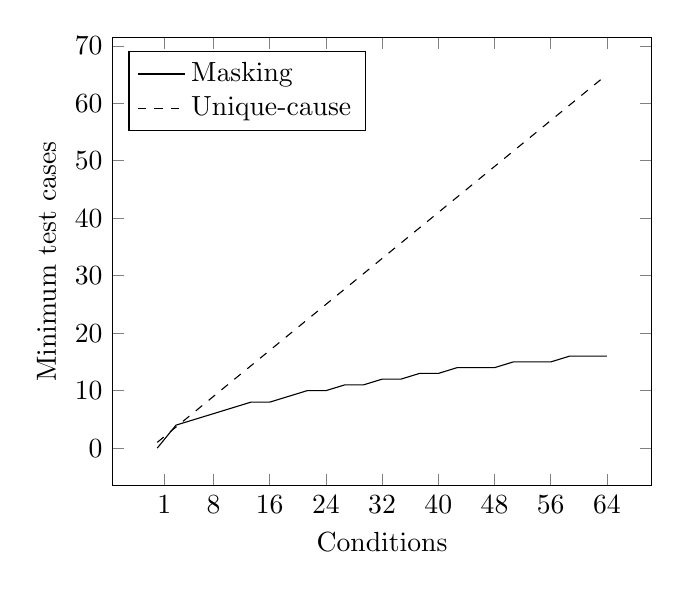
\begin{tikzpicture}
        \begin{axis}[
                domain = 0:64,
                xtick  = {1, 8, 16, ..., 64},
                ytick  = {0, 10, ..., 90},
                xlabel = Conditions,
                ylabel = Minimum test cases,
                legend pos = north west,
                legend cell align = {left},
            ]
            \addplot[] {ceil(2 * sqrt(x)};
                \addlegendentry{Masking}
            \addplot[style = dashed] {x + 1};
                \addlegendentry{Unique-cause}
        \end{axis}
    \end{tikzpicture}

    \pause
    \begin{block}{}
        $N+1 \approx \left \lceil {2\sqrt{N}} \right \rceil$ for small $N$
    \end{block}

\end{frame}

\begin{frame}
    \begin{block}{Nugget}
        Masking MC/DC generally require fewer test cases than unique-cause MC/DC,
        but is as good at detecting errors.
    \end{block}

    \begin{block}{}
        \small{
            Chilenski (2001): An Investigation of Three Forms of the Modified
            Condition Decision Coverage (MCDC) Criterion.
        }
    \end{block}
\end{frame}

\begin{frame}[fragile]
    I wrote a patch for gcc

    \begin{block}{}
        \begin{Verbatim}[fontsize = \footnotesize]
$ git log -n 1 --format=short --shortstat
Author: Jørgen Kvalsvik <jorgen.kvalsvik@woven-planet.global>

    Add condition coverage profiling

21 files changed, 2952 insertions(+), 27 deletions(-)
        \end{Verbatim}
    \end{block}

    \begin{block}{}
        \begin{Verbatim}[fontsize=\footnotesize]
 gcc/tree-profile.cc |  +978
        \end{Verbatim}
    \end{block}
\end{frame}

\begin{frame}
    \begin{block}{Quick start}
        \lstinline{gcc --coverage -fprofile-conditions}
    \end{block}
\end{frame}

\begin{frame}[fragile]
    \begin{block}{Demo}
        \begin{lstlisting}[language = sh, basicstyle = \scriptsize\ttfamily]
$ gcc --coverage -fprofile-conditions
    demo.c -o demo
$ ./demo 0 0 0
$ ./demo 0 0 1
$ ./demo 1 0 0
$ gcov --conditions demo
$ cat demo.c.gcov

    if ((a && b) || c) {
condition outcomes covered 4/6
condition  0 not covered (true)
condition  1 not covered (true)
        \end{lstlisting}
    \end{block}

    \begin{block}{Question}
        Why is \lstinline{a = 1} not covered?
    \end{block}
\end{frame}

\begin{frame}
    \begin{block}{Note}
        This section covers \textbf{masking} MC/DC
    \end{block}
\end{frame}

\begin{frame}
    \begin{block}{Requirement}
        Each basic condition has been shown to \textbf{independently} affect the
        decision’s outcome.
    \end{block}

    \begin{block}{Definition}
        A condition \textbf{independently} affects the outcome if changing it
        while keeping the \textbf{other values constant} changes the outcome.
    \end{block}
\end{frame}

\begin{frame}[fragile]
    \begin{columns}
        \begin{column}{0.5\textwidth}
            \begin{lstlisting}[basicstyle = \footnotesize\ttfamily]
    if ((a && b) || c) {
        //
    } else {
        //
    }
            \end{lstlisting}
        \end{column}

        \begin{column}{0.5\textwidth}
            \begin{tabular}{c c c | c}
                        a & b & c \\
                        \hline
                 \rowhl F & F & F & F \\
                        F & F & T & T \\
                        F & T & F & F \\
                        F & T & T & T \\
                \rowhl  T & F & F & F \\
                        T & F & T & T \\
                        T & T & F & T \\
                        T & T & T & T \\
            \end{tabular}
        \end{column}
    \end{columns}

    \begin{block}{Observation}
        Changing \lstinline{a} does not change the decision
    \end{block}
\end{frame}

\begin{frame}
    This effect is called \emph{masking}

    \begin{itemize}
        \item \lstinline{* || true}
        \item \lstinline{* && false}
    \end{itemize}
\end{frame}

\begin{frame}
    \begin{block}{Commutation}
        Reversing a boolean expression does not change its truth table
        \begin{align*}
            (P \wedge Q) & \equiv (Q \wedge P) \\
            (P \vee Q)   & \equiv (Q \vee P)   \\
        \end{align*}
    \end{block}

    \begin{block}{Observation}
        Masked conditions are \emph{short circuited} in the reversed expression
    \end{block}
\end{frame}

\begin{frame}
    \centering
    \begin{columns}
        \begin{column}{0.3\textwidth}
            \centering
            \lstinline{(a && b) || c}
            \begin{tabular}{c c c | c}
                a & b & c & \\
                \hline
                F & * & F & F \\
                F & * & T & T \\
                F & * & F & F \\
                F & * & T & T \\

                T & F & F & F \\
                T & F & T & T \\
                T & T & * & T \\
                T & T & * & T \\
            \end{tabular}
        \end{column}

        \begin{column}{0.3\textwidth}
            \centering
            \lstinline{c || (b && a)}
            \begin{tabular}{c c c | c}
                c & b & a & \\
                \hline
                F & F & - & F \\
                F & F & - & F \\
                F & T & F & F \\
                F & T & T & T \\

                T & - & - & T \\
                T & - & - & T \\
                T & - & - & T \\
                T & - & - & T \\
            \end{tabular}
        \end{column}
    \end{columns}

    \begin{block}{}
        Short circuiting for the expression * and the reverse -
    \end{block}
\end{frame}

\begin{frame}
    \begin{columns}
        \begin{column}{0.3\textwidth}
            \centering
            \lstinline{(a && b) || c}
            \begin{tabular}{c c c | c}
                a & b & c & \\
                \hline
                F & * & F & F \\
                F & * & T & T \\
                F & * & F & F \\
                F & * & T & T \\

                T & F & F & F \\
                T & F & T & T \\
                T & T & * & T \\
                T & T & * & T \\
            \end{tabular}
        \end{column}

        \begin{column}{0.3\textwidth}
            \centering
            \lstinline{c || (b && a)}
            \begin{tabular}{c c c | c}
                c & b & a & \\
                \hline
                F & F & - & F \\
                T & - & - & T \\
                F & T & F & F \\
                T & - & - & T \\

                F & F & - & F \\
                T & - & - & T \\
                F & T & T & T \\
                T & - & - & T \\
            \end{tabular}
        \end{column}

        \begin{column}{0.3\textwidth}
            \centering
            \lstinline{(a && b) || c}
            \begin{tabular}{c c c | c}
                a & b & c & \\
                \hline
                F & * & F & F \\
                - & - & T & T \\
                F & * & F & F \\
                - & - & T & T \\

                T & F & F & F \\
                - & - & T & T \\
                T & T & * & T \\
                T & T & * & T \\
            \end{tabular}
        \end{column}
    \end{columns}

    \begin{block}{Note}
        Row order in \lstinline{c || (b && a)} changed
    \end{block}
\end{frame}

\newcommand{\rowonly}{%
    \noalign{\ifnum0=`}\fi
    \@rowonly
}
\newcommand<>{\@rowonly}[1]{%
    \only#2%
        {\ifnum0=`{\fi}#1{\ifnum0=`}\fi}%
    \ifnum0=`{\fi}%
    \ignorespaces
}

\begin{frame}
    \centering\lstinline{(a && b) || c}
    \begin{columns}
        \begin{column}{0.4\textwidth}
            \centering
            \begin{tabular}{c c c c | c}
                          & a & b & c & \\
                        \hline
\rowonly<2,4,5>  {\rowhl} 1 & F & * & F & F \\
\rowonly<4,5>    {\rowhl} 2 & - & - & T & T \\
\rowonly<2,4>    {\rowhl} 3 & F & * & F & F \\
\rowonly<4>      {\rowhl} 4 & - & - & T & T \\
\rowonly<2,3,4,5>{\rowhl} 5 & T & F & F & F \\
\rowonly<4>      {\rowhl} 6 & - & - & T & T \\
\rowonly<2,3,5>  {\rowhl} 7 & T & T & * & T \\
\rowonly<2,3>    {\rowhl} 8 & T & T & * & T \\
            \end{tabular}
        \end{column}

        \begin{column}{0.6\textwidth}
            \begin{align*}
              \visible<2>\bullet  &  &      a &= \set{5, 7, 8} \\
              \visible<2>\bullet  &  & \neg a &= \set{1, 3}    \\
              \visible<3>\bullet  &  &      b &= \set{7, 8}    \\
              \visible<3>\bullet  &  & \neg b &= \set{5}       \\
              \visible<4>\bullet  &  &      c &= \set{2, 4, 6} \\
              \visible<4>\bullet  &  & \neg c &= \set{1, 3, 5} \\
            \end{align*}
        \end{column}
    \end{columns}

    \begin{block}{}
        Test sets for cases for masking MC/DC.
    \end{block}
\end{frame}

\begin{frame}
    \begin{block}{Detecting errors}
        \begin{tabular}{l l}
            Specification  & \texttt{(a \&\& b)\quad || c} \\
            Implementation & \texttt{(a \&\& !c) || c} \\
        \end{tabular}
    \end{block}
\end{frame}

\begin{frame}
    \begin{columns}
        \begin{column}{0.3\textwidth}
            \centering
            Masking table
            \begin{tabular}{c c c | c}
                        a & b & c & \\
                        \hline
                        F & * & F & F \\
                        - & - & T & T \\
                        F & * & F & F \\
                        - & - & T & T \\

                        T & F & F & F \\
                        - & - & T & T \\
                        T & T & * & T \\
                        T & T & * & T \\
            \end{tabular}
        \end{column}

        \begin{column}{0.3\textwidth}
            \centering
            \lstinline{(a && !c) || c}
            \only<1> {\begin{tabular}{c c c | c}}%
            \only<2->{\begin{tabular}{c C c | c}}%
                        a & !c & c & \\
                        \hline
                        F & * & F & F \\
                        - & - & T & T \\
                        F & * & F & F \\
                        - & - & T & T \\

                        T & T & * & T \\
                        - & - & T & T \\
                        T & T & * & T \\
                        T & T & * & T \\
            \end{tabular}
        \end{column}
    \end{columns}
\end{frame}

\begin{frame}
    \begin{block}{Note}
        Some strong coupled conditions cannot be detected by masking MC/DC
    \end{block}

    \begin{block}{}
        \lstinline{(a && b) || (a && c)}
    \end{block}{}

    \begin{block}{}
        \begin{columns}
            \begin{column}{0.5\textwidth}
                \centering
                \begin{tabular}{c c c c | c}
            a & b & a & c & \\
            \hline
            0 &         * &         0 &         * & 0 \\
            0 &         * &         0 &         * & 0 \\
            - &         0 &         - & \cellhl 0 & 0 \\
            - & \cellhl 0 & \cellhl 1 & \cellhl 1 & 1 \\
            0 &         * &         - &         0 & 0 \\
    \cellhl 0 &         * & \cellhl 0 &         * & 0 \\
            1 &         1 &         * &         * & 1 \\
    \cellhl 1 & \cellhl 1 &         * &         * & 1 \\
                \end{tabular}
            \end{column}
            \begin{column}{0.5\textwidth}
                Full unique-cause coverage is not possible (\lstinline{a} repeated)
            \end{column}
        \end{columns}
    \end{block}
\end{frame}

\begin{frame}[fragile]
    Cheating MC/DC
    \begin{columns}
        \begin{column}{0.4\textwidth}
            \centering
            \begin{lstlisting}[basicstyle = \footnotesize\ttfamily]
if ((a && b) || c) {
    //
} else {
    //
}
            \end{lstlisting}

        \end{column}

        \begin{column}{0.4\textwidth}
            \centering
            \begin{lstlisting}[basicstyle = \footnotesize\ttfamily]
int ab = a && b;
if (ab || c) {
    //
} else {
    //
}
            \end{lstlisting}
        \end{column}
    \end{columns}

    \begin{columns}
        \begin{column}{0.4\textwidth}
            \centering
            \begin{tabular}{c c c | c}
                        a & b & c \\
                        \hline
                \rowhl  F & F & F & F \\
                \rowhl  F & F & T & T \\
                        F & T & F & F \\
                        F & T & T & T \\
                \rowhl  T & F & F & F \\
                        T & F & T & T \\
                \rowhl  T & T & F & T \\
                        T & T & T & T \\
            \end{tabular}
        \end{column}

        \begin{column}{0.4\textwidth}
            \centering
            \begin{tabular}{c c}
                        ab & c \\
                        \hline
                 \rowhl F & F \\
                        F & T \\
                 \rowhl T & F \\
                 \rowhl T & T \\
            \end{tabular}
        \end{column}
    \end{columns}
\end{frame}

\section{Programs}

\begin{frame}
    \begin{block}{}
        \emph{If computers had blood, we would be considered butchers}
    \end{block}
\end{frame}

\begin{frame}[fragile]
    \begin{block}{}
        gcc does \textbf{control flow graph} analysis for coverage
    \end{block}

    \begin{columns}<2->
        \begin{column}{0.5\textwidth}
            \centering
            \begin{lstlisting}[basicstyle = \scriptsize\ttfamily]
if (a && b && c)
    x = 1;
            \end{lstlisting}
        \end{column}

        \begin{column}{0.5\textwidth}
            \centering
            \begin{lstlisting}[basicstyle = \scriptsize\ttfamily]
if (a)
    if (b)
        if (c)
            x = 1;
            \end{lstlisting}
        \end{column}
    \end{columns}

    \begin{block}<3->
        \centering
        \begin{lstlisting}[basicstyle = \scriptsize\ttfamily]
    #####:    2:    if (a && b && c)
condition outcomes covered 6/6
    #####:    3:        x = 1;

    #####:    2:    if (a)
    #####:    3:        if (b)
    #####:    4:            if (c)
    #####:    5:                x = 1;
condition outcomes covered 6/6
        \end{lstlisting}
    \end{block}
\end{frame}

\begin{frame}[fragile, t]
    \begin{block}{Rust \#1}
        \begin{onlyenv}<1>
            \begin{lstlisting}[basicstyle = \footnotesize\ttfamily]
fn f(a: bool, b: bool, c: bool) -> bool {
    a || (b && c)
}

fn main() {
    f(true,  true, false);
    f(false, true, false);
}
            \end{lstlisting}
        \end{onlyenv}

        \begin{onlyenv}<2>
            \begin{lstlisting}[basicstyle = \scriptsize\ttfamily]
$ gccrs --coverage -fprofile-conditions prog.rs -o prog \
    -frust-incomplete-and-experimental-compiler-do-not-use
$ ./prog
$ gcov --conditions prog
File 'prog.rs'
Lines executed:100.00% of 5
Condition outcomes covered:50.00% of 6
Creating 'prog.rs.gcov'
            \end{lstlisting}
        \end{onlyenv}

        \begin{onlyenv}<3->
            \begin{lstlisting}[
                basicstyle = \scriptsize\ttfamily,
                escapeinside={*@}{@*},
            ]
        2:    1:fn f(a: bool, b: bool, c: bool) -> bool {
        2:    2:    a || (b && c)
condition outcomes covered 3/6*@\tikzmark{summary}{}@*
*@\tikzmark{covered}{}@*condition  1*@\tikzmark{index}{}@* not covered (true false) *@\tikzmark{both-missing}{}@*
condition  2 not covered (tr*@\tikzmark{reports-missing}{}@*ue)
        -:    3:}
        -:    4:
        1:    5:fn main() {
        1:    6:    f(true,  true, false);
        1:    7:    f(false, true, false); *@\tikzmark{bottom}{}@*
        -:    8:}
            \end{lstlisting}

            \begin{tikzpicture}[overlay, remember picture]

                \only<4>{
                    \node (sum) [below of=bottom] {Summary};
                    \draw [->] (sum) to (summary);
                }

                \only<5>{
                    \node (idx) [below of=bottom] {Condition index};
                    \draw [->] (idx) to (index);
                }

                \only<6>{
                    \node (cov) [below of=bottom] {Quiet if fully covered};
                    \draw [->] (cov) to ($(covered) + (0em, 0.5em)$);
                }

                \only<7>{
                    \node (report) [below of=bottom] {
                        Conditions \textbf{not} shown to be independent
                    };
                    \draw [->] (report) to (reports-missing);
                }
            \end{tikzpicture}
        \end{onlyenv}
    \end{block}
\end{frame}

\begin{frame}[fragile, t]
    \begin{block}{Rust \#2}
        \begin{onlyenv}<1>
            \begin{lstlisting}[basicstyle = \scriptsize\ttfamily]
fn loops(init: i32) -> i32 {
    let mut i = init;
    let mut x = 0;
    while true {
        x *= i;
        i += 1;
        if i > 5 { break }
    }
    while i < 20 {
        x -= i;
        i *= 2;
    }
    x
}

fn main() {
    loops(0);
    loops(5);
}
            \end{lstlisting}
        \end{onlyenv}

        \begin{onlyenv}<2>
            \begin{lstlisting}[basicstyle = \tiny\ttfamily]
        2:    1:fn loops(init: i32) -> i32 {
        2:    2:    let mut i = init;
        2:    3:    let mut x = 0;
        5:    4:    while true {
       7*:    5:        x *= i;
condition outcomes covered 1/2
condition  0 not covered (true)
       7*:    6:        i += 1;
condition outcomes covered 1/2
condition  0 not covered (true)
        7:    7:        if i > 5 { break }
condition outcomes covered 2/2
        -:    8:    }
        6:    9:    while i < 20 {
condition outcomes covered 2/2
       4*:   10:        x -= i;
condition outcomes covered 1/2
condition  0 not covered (true)
       4*:   11:        i *= 2;
condition outcomes covered 1/2
condition  0 not covered (true)
        -:   12:    }
        2:   13:    x
        -:   14:}
            \end{lstlisting}
        \end{onlyenv}
    \end{block}
\end{frame}

\begin{frame}[fragile, t]
    \begin{block}{C++ \#1}
        \begin{onlyenv}<1>
            \begin{lstlisting}[basicstyle = \scriptsize\ttfamily]
class C {
public:
    explicit C(int c) noexcept (true) : v(c) {}
    bool operator < (const C& o) const noexcept (true) {
        return this->v < o.v;
    }

private:
    int v;
};

int main() {
    C one(1), two(2);
    int three = 3, four = 4;
    int x = 0;
    if (one < two && four < three)
        x = 1;
}
            \end{lstlisting}
        \end{onlyenv}
        \begin{onlyenv}<2->
            \begin{lstlisting}[basicstyle = \scriptsize\ttfamily]
        1:    9:int main() {
        1:   10:    C one(1), two(2);
        1:   11:    int three(3), four(4);
        1:   12:    int x = 0;
       1*:   13:    if (one < two && four < three)
condition outcomes covered 1/4
condition  0 not covered (true false)
condition  1 not covered (true)
condition outcomes covered 1/2
condition  0 not covered (true)
    #####:   14:        x = 1;
        1:   15:}
            \end{lstlisting}
        \end{onlyenv}
    \end{block}

    \begin{block}{}<3>
        gcc uses a temporary for the \lstinline{if}
    \end{block}
\end{frame}

\begin{frame}[fragile, t]
    \begin{block}{D \#1}
        \begin{lstlisting}[basicstyle = \scriptsize\ttfamily]
        1:    3:void main()
        -:    4:{
        1:    5:    stdin
        -:    6:        .byLineCopy
        -:    7:        .array
        3:    8:        .sort!((a, b) => a > b)
        1:    9:        .each!writeln;
        -:   10:}
        \end{lstlisting}

        \begin{visibleenv}<2->
            string.d.gcov:
            \begin{lstlisting}[basicstyle = \tiny\ttfamily]
        -:  251:    {
        -:  252:        import core.stdc.string : memcmp;
        -:  253:
        5:  254:        const ret = memcmp( s1.ptr, s2.ptr, len );
        5:  255:        if ( ret )
condition outcomes covered 1/2
condition  0 not covered (true)
    #####:  256:            return ret;
        -:  257:    }
        5:  258:    return (s1.length > s2.length) - (s1.length < s2.length);
            \end{lstlisting}
        \end{visibleenv}
    \end{block}
\end{frame}

\begin{frame}[fragile, t]
    \begin{block}{C \#1}
        \begin{lstlisting}[basicstyle = \scriptsize\ttfamily]
        2:    1:int lt(int x, int y) {
        2:    2:    return x < y;
        -:    3:}
        -:    4:
        1:    5:int main() {
        1:    6:    int one = 1, two = 2;
        1:    7:    int three = 3, four = 4;
        1:    8:    int x = 0;
        1:    9:    if (lt(one, two) && lt(four, three))
condition outcomes covered 1/4
condition  0 not covered (true false)
condition  1 not covered (true)
    #####:   10:        x = 1;
        -:   11:}
        \end{lstlisting}
    \end{block}
\end{frame}

\begin{frame}[fragile, t]
    \begin{block}{C \#2}
        \begin{lstlisting}[basicstyle = \scriptsize\ttfamily]
        1:    1:int main() {
        1:    2:    int one = 1, two = 2;
        1:    3:    int three = 3, four = 4;
        1:    4:    int x = 0;
       1*:    5:    int v = one < two && three < four;
condition outcomes covered 2/4
condition  0 not covered (false)
condition  1 not covered (false)
        1:    6:    if (v)
condition outcomes covered 1/2
condition  0 not covered (false)
        1:    7:        x = 1;
        -:    8:    else
    #####:    9:        x = -1;
        -:   10:}
        \end{lstlisting}
    \end{block}
\end{frame}

\begin{frame}[fragile, t]
    \begin{block}{C \#3}
        \begin{lstlisting}[basicstyle = \scriptsize\ttfamily]
        1:    1:int ternary(int a, int b) {
       1*:    2:    int x = (a || b) ? f() : g();
condition outcomes covered 1/4
condition  0 not covered (false)
condition  1 not covered (true false)
        -:    3:}
        \end{lstlisting}
    \end{block}
\end{frame}

\begin{frame}[fragile, t]
    \begin{block}{C \#4}
        \begin{lstlisting}[basicstyle = \scriptsize\ttfamily]
        1:    1:int main() {
        1:    2:    int a = 0, b = 3, c = 2;
        1:    3:    int x = 0;
       1*:    4:    if ((a && b) || (c && a))
condition outcomes covered 2/8
condition  0 not covered (true)
condition  1 not covered (true false)
condition  2 not covered (true false)
condition  3 not covered (true)
    #####:    5:        x = 1;
        \end{lstlisting}
    \end{block}
\end{frame}

\section{Current status}

\begin{frame}
    \begin{itemize}
        \item Condition profiling is currently \textbf{pending review}
        \item Inferring conditionals from the CFG is \textbf{accurate}, but
            sometimes surprising
        \item Approach is sensitive to \textbf{frontend decisions}
        \item Reports can be unwieldy; see \textbf{lcov}
        \item No integration with build systems and testing frameworks
    \end{itemize}
\end{frame}

\section{Algorithm}

\begin{frame}[fragile]
    \begin{columns}
        \begin{column}{0.4\textwidth}
            \begin{lstlisting}[basicstyle = \footnotesize\ttfamily]
if ((a && b) || c) {
    // t
} else {
    // f
}
// e
            \end{lstlisting}
        \end{column}
        \begin{column}{0.4\textwidth}
            \begin{lstlisting}[basicstyle = \footnotesize\ttfamily]
_a:
  if (a) goto _b
  else   goto _c
_b:
  if (b) goto _t
  else   goto _c
_c:
  if (c) goto _t
  else   goto _f
_t:
  goto _e
_f:
  goto _e
_e:
            \end{lstlisting}
        \end{column}
    \end{columns}
\end{frame}

\begin{frame}[fragile]
    \begin{columns}
        \begin{column}{0.4\textwidth}
            \begin{lstlisting}[basicstyle = \footnotesize\ttfamily]
if ((a && b) || c) {
    // t
} else {
    // f
}
// e
            \end{lstlisting}
        \end{column}
        \begin{column}{0.4\textwidth}
            \includegraphics[
                width  = \textwidth,
                height = 0.8\textheight,
                keepaspectratio,
            ]{graph/fig1.pdf}
        \end{column}
    \end{columns}
\end{frame}

\begin{frame}
    \begin{block}{Control flow graph}
        \begin{itemize}
            \item Directed graph
            \item Nodes are an uninterruptible sequence of instructions
            \item Edges are next possible paths of execution
            \item Edges are labelled fallthrough, true/false (conditional), complex
            \item Fallthrough and conditional are mutually exclusive
        \end{itemize}
    \end{block}
\end{frame}

\section{Act I: Inferring decisions}
\begin{frame}[fragile]
    \begin{columns}
        \begin{column}{0.4\textwidth}
            \begin{lstlisting}[basicstyle = \footnotesize\ttfamily]
if ((a && b) || c) {
    // t
} else {
    // f
}
// e
            \end{lstlisting}
        \end{column}
        \begin{column}{0.4\textwidth}
            \includegraphics[
                width  = \textwidth,
                height = 0.8\textheight,
                keepaspectratio,
            ]{graph/fig2.pdf}
        \end{column}
    \end{columns}
\end{frame}

\begin{frame}
    \begin{block}{Observation}
        \begin{equation*}
            \bigcup \set{Succ(v) \mid v \in B} = N[B]
        \end{equation*}
        \begin{equation*}
            N[B] = B \cup O_B
        \end{equation*}

        \begin{tabular}{l l}
            $B$    & is a decision (boolean expression) \\
            $O_B$  & is the \emph{outcome} of $B$ \\
            $N(B)$ & is the \emph{open neighborhood} of $B$ \\
            $N[B]$ & is the \emph{closed neighborhood} of $B$ \\
        \end{tabular}
    \end{block}
\end{frame}

\begin{frame}[fragile]
    \begin{columns}[T]
        \begin{column}{0.6\textwidth}
            \begin{lstlisting}[escapeinside={*@}{@*}, aboveskip = 5em]
if (*@\tikzmark{fst}{}@*(a && b) || c*@\tikzmark{lst}{}@*) {
*@\tikzmark{then}{}@*
} else {
*@\tikzmark{else}{}@*
}
            \end{lstlisting}

            \begin{tikzpicture}[overlay,remember picture]
                \node (fst) at ($(fst) + (0.0em, +1.75ex)$) {};
                \node (lst) at ($(lst) + (0.0em, +1.75ex)$) {};
                \node (top) at ([yshift = 3em]$(fst)!0.5!(lst)$)
                        {uninterruptible};
                \draw [->] (top) to (fst);
                \draw [->] (top) to (lst);

                \node (then) at ($(then) + (5.0em, 0.0em)$) {};
                \node (else) at ($(else) + (5.0em, 0.0em)$) {};
                \node (out) at ($(then)!0.5!(else) + (5.0em, 0.0em)$) {outcome};

                \draw [->] (out) to (then);
                \draw [->] (out) to (else);
            \end{tikzpicture}

            \only<1>{
                \begin{equation*}
                    \bigcup \set{Succ(v) \mid v \in B}
                \end{equation*}
            }

            \only<2>{
                \begin{equation*}
                    E(B) = \set{(u, v) \in E | u \in B, v \in N[B]}
                \end{equation*}
                All edges in $E(B)$ are conditional
            }

            \only<3>{
                \begin{equation*}
                    Succ(B_\Omega) = O_B
                \end{equation*}
            }

            \only<4>{
                Can not goto to/from the middle of an \emph{expression}

                \begin{tikzpicture}[overlay,remember picture]
                    \node (nogoto) at ($(else) + (0.0em, -2.0em)$) {no goto};
                    \draw [->] (nogoto) to ($(fst)!0.5!(lst) + (0.0em, -2.0em)$);
                \end{tikzpicture}
            }
        \end{column}

        \begin{column}{0.4\textwidth}
            \only<1-2>{
                \includegraphics[
                    width  = \textwidth,
                    height = 0.8\textheight,
                    keepaspectratio,
                ]{graph/fig3.pdf}%
            }
            \only<3->{
                \includegraphics[
                    width  = \textwidth,
                    height = 0.8\textheight,
                    keepaspectratio,
                ]{graph/fig4.pdf}%
            }
        \end{column}
    \end{columns}
\end{frame}

\newcommand{\includegraph}[2]{%
    \noindent\includegraphics<#1>[
        width  = \textwidth,
        height = 0.8\textheight,
        keepaspectratio,
    ]{graph/#2.pdf}%
}

\begin{frame}
    Reachable-by-condition-edge (BFS)
\end{frame}

\begin{frame}[fragile]
    \begin{columns}
        \begin{column}{0.4\textwidth}
            \begin{lstlisting}[basicstyle = \footnotesize\ttfamily]
if ((a && b) || c) {
    // t
} else {
    // f
}
            \end{lstlisting}
        \end{column}

        \begin{column}{0.4\textwidth}
            \includegraph{1}{fig5-1}%
            \includegraph{2}{fig5-2}%
            \includegraph{3}{fig5-3}%
            \includegraph{4}{fig5-4}%
            \includegraph{5}{fig5-5}%
            \includegraph{6}{fig5-6}%
            \includegraph{7}{fig5-7}%
            \includegraph{8}{fig5-8}%
            \includegraph{9}{fig5-9}%
            \includegraph{10}{fig5-10}%
            \includegraph{11}{fig5-11}%
        \end{column}
    \end{columns}
\end{frame}

\begin{frame}
    \begin{algorithmic}[1]
        \Function{reach}{$v_0, v_p$}
            \State $R \gets \set{}$
            \State $Q \gets$ \Call {queue}{$v_0$}

            \Repeat
                \State $v \gets$ \Call {pop}{$Q$}
                \ForAll {$s$}{$Succs(v)$}
                    \SkipIf {$s \in R$}
                    \SkipIf {\Call {is-same}{$s, v_p$}}
                    \SkipIf {\Call {is-back-edge}{$v, s$}}
                    \SkipIf {$\neg$ \Call {dominated-by}{$s, v_0$}}
                    \SkipIf {$\neg$ \Call {is-conditional}{$s$}}
                    \State \Call {enqueue} {Q, $s$}
                    \State \Call {add}{$R, s$}
                \EndFor
            \Until{\Call {empty}{$Q$}}
            \State \Return $R$
        \EndFunction
    \end{algorithmic}
\end{frame}

\begin{frame}[fragile]
    \begin{columns}
        \begin{column}{0.4\textwidth}
            \begin{lstlisting}[basicstyle = \footnotesize\ttfamily]
if (a && b) {
    if (c) {
        // p
    } else {
        // q
    }
} else {
    // r
}
            \end{lstlisting}
        \end{column}

        \begin{column}{0.5\textwidth}
            \includegraph{1}{fig6-1}%
            \includegraph{2}{fig6-2}%
            \includegraph{3}{fig6-3}%
            \includegraph{4}{fig6-4}%
            \includegraph{5}{fig6-5}%
        \end{column}
    \end{columns}
\end{frame}

\begin{frame}[fragile]
    \begin{columns}
        \begin{column}{0.5\textwidth}
            \begin{lstlisting}[basicstyle = \footnotesize\ttfamily]
if (a && b) {
    if (c) {
        // p
    } else {
        // q
    }
} else {
    // r
}
            \end{lstlisting}
            \begin{equation*}
                C = (\textcolor{dotlightblue}{G}, \textcolor{dotlightcoral}{G'})
            \end{equation*}
            \begin{equation*}
                \begin{split}
                    \forall_e \in E(G) & \bullet cond(e) \\
                    \Rightarrow & O_B \subset N[G] \\
                    \Rightarrow & B \subseteq G
                \end{split}
            \end{equation*}
        \end{column}

        \begin{column}{0.5\textwidth}
            \includegraphics[
                width   = \linewidth,
                height  = 0.8\textheight,
                keepaspectratio,
            ]{graph/fig7.pdf}
        \end{column}
    \end{columns}
\end{frame}

\begin{frame}[fragile]
    \begin{columns}
        \begin{column}{0.5\textwidth}
            \begin{lstlisting}[
                basicstyle = \footnotesize\ttfamily,
                escapeinside={*@}{@*},
                aboveskip = 5em,
            ]
if (*@\tikzmark{a}{}@*a && *@\tikzmark{b}{}@*b) {*@\tikzmark{open}{}@*
    if (c) {*@\tikzmark{c}{}@*
        // p*@\tikzmark{p}{}@*
    } else {*@\tikzmark{right}{}@*
        // q*@\tikzmark{q}{}@*
    }
} else {
    // r*@\tikzmark{r}{}@*
}
*@\tikzmark{e}{}@*
            \end{lstlisting}

            \begin{tikzpicture}[overlay,remember picture]
                \coordinate (top) at ($(b) + (2.0em, 2.0em)$) {};
                \coordinate (right) at ($(right) + (+4.0em, 0.0em)$) {};
                \node (a) at (a.{north east}) {};
                \draw [->, blue]
                    (a)     to [bend left = 30]
                    (top)   to [bend left = 40]
                    (right) to [bend left = 45]
                    (r)
                ;

                \draw [->, blue]
                    (a)                         to [bend left = 30]
                    ($(top)  + (0em, 1em)$)     to [bend left = 60]
                    ($(open) + (2em, 0em)$)     to [bend left = 40]
                    (c.{north east})
                ;

                \node (b) at (b.{north east}) {};
                \coordinate (top) at ($(top) + (2.0em, 0.0em)$) {};
                \coordinate (right) at ($(right) + (+2.0em, 0.0em)$) {};
                \draw [->, purple]
                    (b)     to [bend left = 30]
                    (top)   to [bend left = 40]
                    (right) to [bend left = 60]
                    (r.{south})
                ;

                \draw [->, purple]
                    (b)                         to [bend left = 40]
                    ($(top)  + (0em, 1em)$)     to [bend left = 60]
                    ($(open) + (3em, 0em)$)     to [bend left = 40]
                    (c.{east})
                ;

            \end{tikzpicture}
            No path from \textbf{then} to \textbf{else}
        \end{column}

        \begin{column}{0.5\textwidth}
            \noindent\includegraphics[
                width  = \textwidth,
                height = 0.8\textheight,
                keepaspectratio,
            ]{graph/fig8.pdf}
        \end{column}
    \end{columns}
\end{frame}

\begin{frame}[fragile]
    \begin{columns}
        \begin{column}{0.5\textwidth}
            \begin{lstlisting}[
                basicstyle = \footnotesize\ttfamily,
                escapeinside={*@}{@*},
                aboveskip = 1em,
            ]
if (a && b) {*@\tikzmark{top}{}@*
    if (c) {
        // p
    } else {
        // q
    }
} else {*@\tikzmark{bot}{}@*
    // r
}
            \end{lstlisting}

            \visible<2->{
                \begin{tikzpicture}[overlay,remember picture]
                    \node (top) at (top) {};
                    \node (bot) at (bot) {};
                    \node (mid) at ($(top)!0.5!(bot) + (+5.0em, 0.0em)$)
                        {outcome};
                    \draw [->] (mid.{north west}) to (top);
                    \draw [->] (mid.{south west}) to (bot);
                \end{tikzpicture}
            }

            \alt<1-2>{
                \begin{equation*}
                    \begin{split}
                        \forall_v \in then(B) \bullet B \subset A(v) \\
                        \forall_v \in else(B) \bullet B \subset A(v) \\
                    \end{split}
                \end{equation*}
                where $A(v)$ are the ancestors of $v$
            }{
                \begin{align*}
                    B &= A_G(v_T) = A_G(v_F) \\
                        &= \bigcap \set { A_G(v) \mid v \in N(G)} \\
                \end{align*}
                where
                \begin{tabular}{l}
                    $A_G(v) = A(v) \cap G$ \\
                    $\set{ v_T, v_F } = O_B$ \\
                \end{tabular}
            }
        \end{column}

        \begin{column}{0.5\textwidth}
            \noindent\includegraphics[
                width  = \textwidth,
                height = 0.8\textheight,
                keepaspectratio,
            ]{graph/fig8.pdf}
        \end{column}
    \end{columns}
\end{frame}

\begin{frame}[fragile]
    \begin{columns}
        \begin{column}{0.5\textwidth}
            \begin{lstlisting}[
                basicstyle = \footnotesize\ttfamily,
            ]
    if (a && b) {
        if (c) // p
        else   // q
    } else {
        // r
    }
            \end{lstlisting}

            \setbeamercovered{invisible}
            \begin{align*}
                    \onslide<2->
                    \disponslide{2-}{A(q)}  & \disponslide{2-}{= \set{c, b, a}} \\
                    \disponslide{3-}{A(p)}  & \disponslide{3-}{= \set{c, b, a}} \\
                    \disponslide{4-}{A(r)}  & \disponslide{4-}{= \set{b, a}   } \\
                    \disponslide{5-}{B}     & \disponslide{5-}{= \bigcap \set{A(q), A(p), A(r)}} \\
                    \disponslide{5-}{}      & \disponslide{5-}{= \set{a, b}} \\
                    \disponslide{5-}{O_B}   & \disponslide{5-}{= \set{r, c}} \\
            \end{align*}
        \end{column}

        \begin{column}{0.5\textwidth}
            \includegraph{1}{fig9-1}%
            \includegraph{2}{fig9-2}%
            \includegraph{3}{fig9-3}%
            \includegraph{4}{fig9-4}%
            \includegraph{5-}{fig9-5}%
        \end{column}
        \setbeamercovered{}
    \end{columns}
\end{frame}

\begin{frame}
    \begin{block}{Problem}
        BFS needs to start at left-most term $B_0$
    \end{block}

    \begin{block}{Solution}
        Process program depth-first, mark when processed
    \end{block}

    \begin{itemize}
        \item If $v$ is fallthrough $\Rightarrow$ mark and continue
        \item If $v$ is conditional $\Rightarrow$ is $B_0$ and $B$ are marked
        \item If $v$ is marked $\Rightarrow$ continue
    \end{itemize}

    \begin{block}{Note}
        May lead to expressions being processed "out of order"
    \end{block}
\end{frame}

\begin{frame}
    \begin{algorithmic}[1]
        \Function{find-decision}{$v_0, v_p$}
            \State $G \gets$ \Call {reach}{$v_0, v_p$}
            \If {$|G| = 1$}
                \State \Return $G$
            \EndIf

            \State $B \gets G$
            \ForAll{$n$}{$N(G)$}
                \State $P \gets \set{}$
                \ForAll{$v$}{$Preds(n)$}
                    \State $P \gets P\ \cup$ $A_G(v)$
                \EndFor
                \State $B \gets B \cap P$
            \EndFor

            \State \Return $B$
        \EndFunction
    \end{algorithmic}
\end{frame}

\begin{frame}[fragile]
    \begin{lstlisting}[
        basicstyle = \scriptsize\ttfamily,
        language = c++,
    ]
cond_reachable_from (p, post, reachable, G);
if (G.length () == 1) {
    out.safe_push (p);
    return;
}

neighborhood (G, reachable, NG);
bitmap_copy (expr, reachable);

for (const basic_block neighbor : NG) {
    bitmap_clear (ancestors);
    for (edge e : neighbor->preds)
        ancestors_of (e->src, p, reachable, ancestors);
    bitmap_and (expr, expr, ancestors);
}

for (const basic_block b : G)
    if (bitmap_bit_p (expr, b->index))
        out.safe_push (b);
out.sort (cmp_index_map, &ctx.index_map);
    \end{lstlisting}
\end{frame}

\begin{frame}
    \begin{algorithmic}[1]
        \Function{find-all-decisions}{$G$}
            \State $R \gets \set{}$

            \For {$v_0 \gets$ \Call {depth-first}{$G$}}
                \SkipIf {\Call {marked}{$v_0$}}

                \If {\Call {is-conditional}{$v_0$}}
                    \State $v_p \gets$ \Call {get-post-dominator}{$v_0$}
                    \State $B \gets$ \Call {find-decision}{$v_0, v_p$}
                    \State \Call {add}{$R, B$}
                    \State \Call {mark}{$B$}
                \Else
                    \State \Call {mark}{$v_0$}
                \EndIf
            \EndFor
            \State \Return $R$
        \EndFunction
    \end{algorithmic}
\end{frame}

\section{Act II: The masking vector}

\begin{frame}[fragile]
    \begin{block}{When masking happens}
        \lstinline{* || true}

        \lstinline{* && false}
    \end{block}
\end{frame}

\begin{frame}[fragile]
    \begin{block}{Observation}
        Boolean expression are are isomorphic under the operator

        \begin{columns}
            \begin{column}{0.4\textwidth}
                \centering
                \includegraphics[
                    width   = 0.8\textwidth,
                    height  = 0.8\textheight,
                    keepaspectratio,
                ]{graph/fig10-1.pdf}
                \lstinline{a || b}
            \end{column}
            \begin{column}{0.4\textwidth}
                \centering
                \includegraphics[
                    width   = 0.8\textwidth,
                    height  = 0.8\textheight,
                    keepaspectratio,
                ]{graph/fig10-2.pdf}
                \lstinline{a && b}
            \end{column}
        \end{columns}
    \end{block}
\end{frame}

\begin{frame}
    \begin{block}{Proposition}
        Boolean expression are are isomorphic under the operator
    \end{block}

    \begin{block}{Proof}
        De Morgan's Laws
        \begin{align*}
            \neg(P \wedge Q) & \equiv \neg P \vee \neg Q \\
            \neg(P \vee Q) & \equiv \neg P \wedge \neg Q \\
        \end{align*}
    \end{block}

    \begin{block}{Implication}
        We don't need to know the operator, only the graph shape
    \end{block}
\end{frame}

\begin{frame}[fragile]
    \begin{block}{When masking happens (in CFG)}
        When a value $c$ is changed (taking a different edge at $v_c$) and
        we still end in the same outcome node
    \end{block}

    \lstinline{f = a || b}

    \begin{columns}
        \begin{column}{0.3\textwidth}
            \centering
            \includegraphics[
                width  = \linewidth,
                height = \textheight,
                keepaspectratio,
            ]{graph/fig11-1.pdf}
            \lstinline{f 1 0}
        \end{column}

        \begin{column}{0.3\textwidth}
            \centering
            \includegraphics[
                width  = \linewidth,
                height = \textheight,
                keepaspectratio,
            ]{graph/fig11-2.pdf}
            \lstinline{f 1 1}
        \end{column}

        \begin{column}{0.3\textwidth}
            \centering
            \includegraphics[
                width  = \linewidth,
                height = \textheight,
                keepaspectratio,
            ]{graph/fig11-3.pdf}
        \lstinline{f 0 1}
        \end{column}
    \end{columns}
\end{frame}

\begin{frame}
    \begin{block}{Observation}
        Masking happens at nodes with \emph{multiple} predecessors
    \end{block}

    \begin{block}{Implication}
        Multiple predecessors means short circuiting edge
    \end{block}

    \begin{block}{Implication}
        We know where to start searching
    \end{block}
\end{frame}

\begin{frame}
    \begin{block}{Association}
        \begin{align*}
            P \wedge (Q \wedge R) & \equiv (P \wedge Q) \wedge R \\
            P \vee (Q \vee R) & \equiv (P \vee Q) \vee R \\
        \end{align*}
    \end{block}

    \begin{block}{Implication}
        We can re-write expressions to an \emph{alternating} form

        \begin{align*}
            (A \vee B) \vee ((C \wedge D) \vee E) \\
            A \vee B \vee (C \wedge D) \vee E     \\
        \end{align*}
    \end{block}
\end{frame}

\begin{frame}
    \begin{block}{Observation}
        Masking propagates until the operator changes
    \end{block}

    \begin{block}{}
        \begin{equation*}
            A \wedge (B \vee C \vee D)
        \end{equation*}

        $D = t$ masks $B$, $C$, but not $A$
    \end{block}
\end{frame}

\begin{frame}
    \begin{block}{Subexpressions can mask}
        \begin{equation*}
            A \wedge (B \vee C)
        \end{equation*}
        $C = f$ masks $A$, but not $B$

        \begin{equation*}
            F = B \vee C
        \end{equation*}
        \begin{equation*}
            A \wedge F
        \end{equation*}
    \end{block}
\end{frame}

\begin{frame}
    \begin{block}{Observation}
        The \emph{last term} $S_\Omega$ in a subexpression can short circuit
        the superexpression
    \end{block}
\end{frame}

\begin{frame}
    \begin{equation*}
            a \wedge b
        \wedge
            (c \vee d)
        \wedge
            e \wedge f
        \wedge
            (g
            \vee
                (h \wedge i)
            \vee
            j)
        \wedge
            k
    \end{equation*}

    \begin{tikzpicture}[node distance = 2em]
        \node (o1)               {$\wedge$};
        \node (o2) [below of=o1] {$\vee$};
        \node (o3) [below of=o2] {$\wedge$};

        \node (a)  [right of=o1] {$a$};
        \node (b)  [right of=a]  {$b$};
        \node (1)  [right of=b]  {};
        \node (c)  [below of=1]  {$c$};
        \node (d)  [right of=c]  {$d$};
        \node (2)  [above of=d]  {};
        \node (e)  [right of=2]  {$e$};
        \node (f)  [right of=e]  {$f$};
        \node (3)  [right of=f]  {};
        \node (g)  [below of=3]  {$g$};
        \node (4)  [right of=g]  {};
        \node (h)  [below of=4]  {$h$};
        \node (i)  [right of=h]  {$i$};
        \node (6)  [right of=i]  {};
        \node (j)  [above of=6]  {$j$};
        \node (7)  [right of=j]  {};
        \node (k)  [above of=7]  {$k$};
        \node (x)  [right of=k]  {};

        \onslide<2>{
            \draw [->] (c.{north}) to [bend left  = 30] (e.{west});
            \draw [->] (h.{north}) to [bend left  = 30] (j.{west});
        }

        \onslide<3>{
            \draw [->] (d.{north}) to [bend left  = 30] (e.{west});
        }

        \onslide<4->{
            \draw [->] (d.{north}) to [bend left  = 45] (x.{north west});
        }
        \onslide<5->{
            \draw [->] (d.{north}) to [bend right = 45] (a.{north east});
            \draw [->] (d.{north}) to [bend right = 30] (b.{east});
        }
    \end{tikzpicture}

    \begin{block}{}
            \only<1> {\phantom{$c = true$}}
            \only<2> {$c = true, h = true$}
            \only<3> {$d = true$}
            \only<4->{$d = false$}
    \end{block}
\end{frame}

\begin{frame}
    \begin{equation*}
        Succ(B_\Omega) = O_B
    \end{equation*}

    \begin{block}{Observation}
        On evaluating a condition; either
        \begin{itemize}
            \item Short-circuit right operands
            \item Evaluate next operand
        \end{itemize}
    \end{block}

    \begin{block}{Implication}
        If one edge is a short circuiting edge, the other must be a masking
        edge
    \end{block}
\end{frame}

\begin{frame}
    \begin{block}{Problem}
        Given a pair of incoming edges, which is masking and which is short
        circuting?
    \end{block}

    \begin{block}{Proposition}
        An ordering $v_n < v_m$ if $v_n$ is a left operand and $v_m$ is
        a right operand in the same expression
    \end{block}

    \begin{block}{Solution}<2>
        Topological sort
    \end{block}
\end{frame}

\begin{frame}
    Given $\set{v_n, v_m} = Preds(v), v_n < v_m$ then
    \begin{align*}
        v_n &= S_\Omega \\
        O_S &= Succ(v_n) \\
    \end{align*}
    where $S$ is a subexpression of $B$ ($S \subset B$)

    \begin{block}{Implication}
        When $(v_m, v)$ is taken, $S$ are masked
    \end{block}
\end{frame}

\begin{frame}
    \begin{columns}
        \begin{column}{0.5\textwidth}
            \begin{align*}
                { v_n, v_m } &= Preds(v) \\
                v_n &= S_\Omega \\
                O_S &=  Succ(v_n) \\
            \end{align*}
        \end{column}

        \begin{column}{0.5\textwidth}
            \begin{block}{Remember}
                \begin{align*}
                    N[B] &= \bigcup \set{Succ(v) \mid v \in B} \\
                    N(B) &= O_B \\
                \end{align*}
            \end{block}

            Everything that applies to the superexpression $B$ applies to the
            subexpression $S$
        \end{column}
    \end{columns}
\end{frame}

\begin{frame}
    \begin{block}{Problem}
        Given a node $v$ with $|Preds(v)| \geq 2$, find the nodes masked when
        taking an edge to $v$
    \end{block}

    \begin{block}{Intermediate problem}
        There can be more than one masking edge
    \end{block}

    \begin{block}{Solution}
        \begin{equation*}
            \set{(v_n, v_m) \in Preds(v) \times Preds(v) \mid v_n < v_m}
        \end{equation*}
    \end{block}
\end{frame}

\begin{frame}[fragile]
    \begin{columns}
        \begin{column}{0.5\textwidth}
            \centering
            \begin{equation*}
                \set{(v_n, v_m) \in Preds(v)^2 \mid v_n < v_m}
            \end{equation*}
            \lstinline{a && b && c}
        \end{column}

        \begin{column}{0.5\textwidth}
            \includegraph{1}{fig12-1}%
            \includegraph{2}{fig12-2}%
            \includegraph{3}{fig12-3}%
            \includegraph{4}{fig12-4}%
        \end{column}
    \end{columns}
\end{frame}

\begin{frame}
    \begin{block}{Remember}
        \begin{align*}
            N[S] &= \bigcup \set{Succ(v) \mid v \in S} \\
            N(S) &= O_S \\
        \end{align*}
    \end{block}
    \begin{block}{Implication}
        \begin{align*}
            Succs(v_k) \subset S_n & \Rightarrow S_{n+1} = S_n \cup
            \set{v_k} \\
            S_0 &= O_S \\
            S   &= S^f - S_0 \\
        \end{align*}
        where $S^f$ is the fixed point $S_{n+1} = S_n$
    \end{block}
\end{frame}

\begin{frame}[fragile]
    \begin{columns}
        \begin{column}{0.6\textwidth}
            \centering
            \lstinline{A && ((B && C) || D)}
            \onslide<3->{
                \begin{tabular}{l l}
                    $(c, t)$ & short circuits \\
                    $(d, t)$ & masks \\
                    $c < d$ \\
                \end{tabular}
            }
            \begin{align*}
                \disponslide{4-}{S_\Omega} & \disponslide{4-}{= c} \\
                \disponslide{4-}{O_S} & \disponslide{4-}{= Succ(c) = \set{d, t}}  \\
                \disponslide{5-}{S_0} & \disponslide{5-}{= d, t} \\
                \disponslide{6-}{S_1} & \disponslide{6-}{= S_0 + c = \set{d, t, c}} \\
                \disponslide{7-}{S_2} & \disponslide{7-}{= S_1 + b = \set{d, t, c, b}} \\
                \disponslide{7-}{S^f} & \disponslide{7-}{= S_2} \\
                \disponslide{8-}{S}   & \disponslide{8-}{= S^f - O_S} \\
                \disponslide{8-}{S}   & \disponslide{8-}{=\set{b, c}} \\
            \end{align*}
        \end{column}

        \begin{column}{0.4\textwidth}
            \includegraph{1}{fig13-1}%
            \includegraph{2}{fig13-2}%
            \includegraph{3}{fig13-3}%
            \includegraph{4}{fig13-4}%
            \includegraph{5}{fig13-5}%
            \includegraph{6}{fig13-6}%
            \includegraph{7}{fig13-7}%
            \includegraph{8-}{fig13-8}%
        \end{column}
    \end{columns}
\end{frame}

\begin{frame}
      \begin{algorithmic}[1]
      \Function{masking-vector}{$B$}
          \State $M \gets \set{}$
          \ForAll {$b$}{$B \cup O_B$}
              \ForAll{$(u, v)$}{$\set{(u, v) \mid Pred(b)^2, u < v}$}
                  \State $Q \gets$ \Call {queue}{$u$}
                  \State \Call {mark}{$Succ(u)$}

                  \Repeat
                      \State $q \gets$ \Call {pop}{$Q$}
                      \SkipIf {\Call {marked}{$Succ(q)$}}
                      \State \Call {mark}{$q$}
                      \State \Call {add}{$M(v, b), q$}

                      \ForAll {$p$}{$Pred(q)$}
                          \SkipIf {$\neg$ \Call {is-conditional} {$p$}}
                          \SkipIf {\Call {is-back-edge}{$q, p$}}
                          \SkipIf {\Call {marked}{$p$}}
                          \SkipIf {$p \not \in B$}
                          \State \Call {enqueue}{$Q, p$}
                      \EndFor

                  \Until {\Call {empty}{Q}}
              \EndFor
          \EndFor
          \State \Return $M$
      \EndFunction
  \end{algorithmic}
\end{frame}

\section{Act III: Instrumentation}

\begin{frame}
    Instrumentation must be fast
\end{frame}

\begin{frame}
    \begin{block}{Remember}
        There is an ordering $v_n < v_m$ if $v_n$ is a left operand and $v_m$ is
        a right operand in the same expression
    \end{block}

    \begin{block}{Implication}
        We can sort $B$
    \end{block}

    \begin{block}{Implication}
        There is a bijection $f: B \rightarrow \mathbb{N}$
    \end{block}
\end{frame}

\begin{frame}[fragile]
    \begin{block}{Global accumulators}
        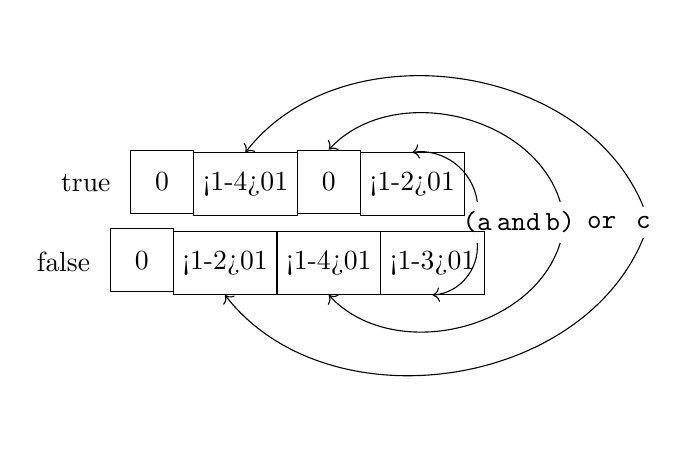
\begin{tikzpicture}
            \matrix (T) [
                matrix of nodes,
                nodes={draw, minimum size=8mm},
                column sep=-\pgflinewidth,
                label = left:true,
            ]{
                0 &
                \alt<1-4>{0}{1} &
                0 &
                \alt<1-2>{0}{1} \\
            };
            \matrix (F) [
                matrix of nodes,
                nodes={draw, minimum size=8mm},
                column sep=-\pgflinewidth,
                label = left:false,
                below of = T
            ]{
                0 &
                \alt<1-2>{0}{1} &
                \alt<1-4>{0}{1} &
                \alt<1-3>{0}{1} \\
            };

            \coordinate (anchor) at ($(T)!0.5!(F) + (+5.0em, 0.0em)$) {};
            \node (a) [node distance = 1.5em, right of=anchor] {\ttfamily (a};
            \node (1) [node distance = 1.5em, right of=a]      {\ttfamily and};
            \node (b) [node distance = 1.5em, right of=1]      {\ttfamily b)};
            \node (2) [node distance = 1.5em, right of=b]      {\ttfamily or};
            \node (c) [node distance = 1.5em, right of=2]      {\ttfamily c};

            \onslide<2->{
                \draw [->] (c.{north}) to [bend right = 60] (T-1-2.{north});
                \draw [->] (c.{south}) to [bend left  = 60] (F-1-2.{south});
                \draw [->] (b.{north}) to [bend right = 60] (T-1-3.{north});
                \draw [->] (b.{south}) to [bend left  = 60] (F-1-3.{south});
                \draw [->] (a.{north}) to [bend right = 45] (T-1-4.{north});
                \draw [->] (a.{south}) to [bend left  = 45] (F-1-4.{south});
            }
        \end{tikzpicture}

        \begin{tabular}{l}
            \visible<3->{\lstinline{f 0 0 1}} \\
            \visible<4->{\lstinline{f 0 0 0}} \\
            \visible<5->{\lstinline{f 1 0 0}} \\
        \end{tabular}
    \end{block}
\end{frame}

\begin{frame}
    \begin{block}{Local accumulators}
        \begin{align*}
            acc & \gets acc \cup B(E(u, v)) \\
            acc & \gets acc \cap M(E(u, v)) \\
        \end{align*}

        where $E(u, v)$ is the edge taken and $M(E)$ are nodes masked for $E$
    \end{block}

    \begin{block}{Remember}
        There is bijection $f: B \rightarrow \mathbb{N}$
    \end{block}
\end{frame}

\begin{frame}[fragile]
    \centering
    \lstinline{a || b}
    \begin{columns}
        \begin{column}{0.3\textwidth}
            \begin{lstlisting}[language=C, basicstyle=\small\ttfamily]
_prelude_fn:
  _t = {0}
  _f = {0}
_a:
  if (a)
    _t |= 0x01
    goto _T
  else
    _f |= 0x01
    goto _b
            \end{lstlisting}
        \end{column}

        \begin{column}{0.3\textwidth}
        \begin{lstlisting}[language=C, basicstyle=\small\ttfamily]
_b:
  if (b)
    _t &= 0x01
    _f &= 0x01
    _t |= 0x02
    goto _T
  else
    _f |= 0x02
    goto _F
        \end{lstlisting}
        \end{column}

        \begin{column}{0.3\textwidth}
            \begin{lstlisting}[language=C, basicstyle=\small\ttfamily]
_T:
  goto _E
_F:
  goto _E
_E:
  _fn_t |= _t
  _fn_f |= _f
        \end{lstlisting}
        \end{column}
    \end{columns}
\end{frame}

\begin{frame}
    \begin{columns}
        \begin{column}{0.5\textwidth}
            Local accumulators are flushed (bitwise-or) on edge-to-outcome
        \end{column}

        \begin{column}{0.5\textwidth}
            \includegraphics[
                width   = \linewidth,
                height  = 0.8\textheight,
                keepaspectratio]{graph/fig14.pdf}
        \end{column}
    \end{columns}
\end{frame}

\begin{frame}
    \centering{\Large{Thank you}}
    \begin{columns}
        \begin{column}[T]{0.5\textwidth}
            \begin{block}{Me}
                \begin{description}
                    \item [Who] Jørgen Kvalsvik
                    \item [How] \lstinline{<j@lambda.is>}
                    \item [Where] Woven by Toyota in Tokyo, Japan
                \end{description}
            \end{block}
        \end{column}

        \begin{column}[T]{0.5\textwidth}
            \begin{block}{Resources}
                \begin{description}
                    \item [Hayhurst (2001)] A Practical Tutorial on Modified
                        Condition/ Decision Coverage.
                    \item [Chilenski (2001)] An Investigation of Three Forms of
                        the Modified Condition Decision Coverage (MCDC)
                        Criterion.
                \end{description}
            \end{block}
        \end{column}
    \end{columns}
\end{frame}

\end{document}
